\documentclass[12pt]{article}

\usepackage{amsmath}    % need for sub-equations
\usepackage{graphicx}   % need for figures
\usepackage{verbatim}   % useful for program listings
\usepackage{color}      % use if color is used in text
\usepackage{subfigure}  % use for side-by-side figures
\usepackage{hyperref}   % use for hypertext links, including those to external 
\usepackage{minted}
\usepackage{listings}
% \usepackage[showframe]{geometry} % remove gay indentation 
% \usepackage{gensymb} % allows me to use fancy symbols in-text


\usepackage{graphicx} % use for images
\graphicspath{ {./images/} } % set path used for images

\setlength{\baselineskip}{16.0pt}    % 16 pt usual spacing between lines

\setlength{\parskip}{3pt plus 2pt}
\setlength{\parindent}{20pt}    
\setlength{\oddsidemargin}{0.5cm}
\setlength{\evensidemargin}{0.5cm}
\setlength{\marginparsep}{0.75cm}
\setlength{\marginparwidth}{2.5cm}
\setlength{\marginparpush}{1.0cm}
\setlength{\textwidth}{150mm}
\linespread{1.25}


 \begin{comment}
    \pagestyle{empty} % doesn't count for page numbers
 \end{comment}
        
        
\begin{document}
        
        \author{Candiate code: hjk123}            \begin{titlepage}
                \begin{center}
                  % \small{Mathematics SL, IA:} \\
                \Huge{A Mathematical Exploration of the \\ Decay of Caffeine}
                \break
                {\large A Mathematics Internal Assessment}
                \break                    %\small{Written by Johan-Petter R. Dragic}
                 % \date{06.11.2018}
                    
        
                    % ADD BREAK HERE
                \vspace{12mm}
                
\includegraphics[scale=0.38]{coffee1.jpg}
                % source pic:http://www.mobileswall.com/wallpaper/coffee-beans-in-a-coffee-cup-free/            
    
            \end{center}
                    \end{titlepage}
        
            \tableofcontents
            \thispagestyle{empty}
            \addtocounter{page}{-1}
            
        %     Structure:
        %             1. Introduction
        %                 purpose and aim, personal engagement
        %             2. Collection of data
        %                 Experimental methods
                                % Simulation



            %%%%%%%%%%%%%%%%%%%%%%%%%%%%%    START OF DOCUMENT    %%%%%%%%%%%%%%%%%%%%%%%%%%%%%%%%%%%%%%%% 
            \newpage
            \section{Introduction} % and personal engagement
            \paragraph{}
                Coffee has become an integral part of many lives, including mine. It's what wakes you up in the morning and sustains your energy-levels throughout the day. The leading chemical stimulant in coffee is called caffeine and it's classified as a "Psychoactive drug", meaning that it alters the chemical processes that goes on in your brain. The main effect of caffeine is to alter the brain's perception of when it's tired, and is the reason why I and many others admire this mild drug. And since the world average amount of sleep lies bellow the hourly optimum, it is no wonder why caffeine consumed to such extents as it is today.
                \\
                Due to the psychoactive effects of caffeine on tiredness many advice to not drink caffeine-containing beverages 3 hours before bed, but how did they come to this conclusion?
                


                \noindent The purpose of this math IA is therefore to explore the decay of caffeine with the aim of figuring out how early before bed you can dink your last cup of coffee without it affecting your sleep.



        \section{Data collection}
        \paragraph{}
                Much like radioactive elements in physics, caffeine follows the same pattern that alpha decay does, meaning that it has a half-life. A Half-life in the realm of nuclear physics is defined as time taken for the radioactive activity of an element to halve itself. So if we were to have a sample of the element Plutonium-238 has an initial activity of $1$ and a half life of 2 hours. Then if you then wait for 2 hours, the activity is now going to be {$\frac{1}{2}$}. I have therefore concluded to use computer simulations as my data collection, and since there are no available simulations specifically for caffeine I will collect data from a simple python program which will apply the principles of the half-life (Raw code is attached to the appendix). 

                \noindent To obtain the half-life of caffeine a search of scholarly articles have been conducted. A study preformed by the American Society of Health-System Pharmacists has found that the half-life of caffeine lies varies between 3 to 5 hours in adults. 
                %%%%%
                %% Source: [American Society of Health-System Pharmacists 2013; Drug Information 2013. Bethesda, MD. 2013, p. 2569] 
                %% https://toxnet.nlm.nih.gov/cgi-bin/sis/search2/r?dbs+hsdb:@term+@rn+58-08-2
                %%%%%
                This is subject to errors made by the original writer but for the sake of this exploration we will assume that his findings hold true. 
                
                \noindent
                Since he aim of this exploration is  to determine how early before bed you can drink your last cup of coffee, we will take assume that the person drinking is at the lower echelon of caffeine decomposition, and caffeine wil therefore have a half-life of \textit{5 hours}. 
                
                \noindent the table bellow shows the simulation output. A note to the data is that the simulation will not calculate for values down to the absolute 0, but rather down do a 0 value of 0.01 (15 data points). This is due to the nature of Mathematics when continuously dividing. (the last output of the simulation before it returned 0.0 was $4.95\times 10^-324$)

                % Inserting table
                \begin{center}
                        \begin{tabular}{cc}
                        Time (h) & mg of caffeine       \\
                        0 & 100  \\ 
                        1 & 50.0  \\ 
                        2 & 25.0   \\
                        3 & 12.5    \\ 
                        4 & 6.25     \\ 
                        5 & 3.13      \\ 
                        6 & 1.56       \\
                        7 & 0.781       \\
                        8 & 0.391        \\
                        9 & 0.195         \\ 
                        10 & 0.0977        \\ 
                        11 & 0.0488         \\ 
                        12 & 0.0244          \\ 
                        13 & 0.0122           \\
                        14 & 0.00610           \\
                        
                                           
                        \end{tabular}
                        
                \end{center}
                
                The data above can be plotted on a scatter-graph and is shown below.
                
                \begin{center}
                        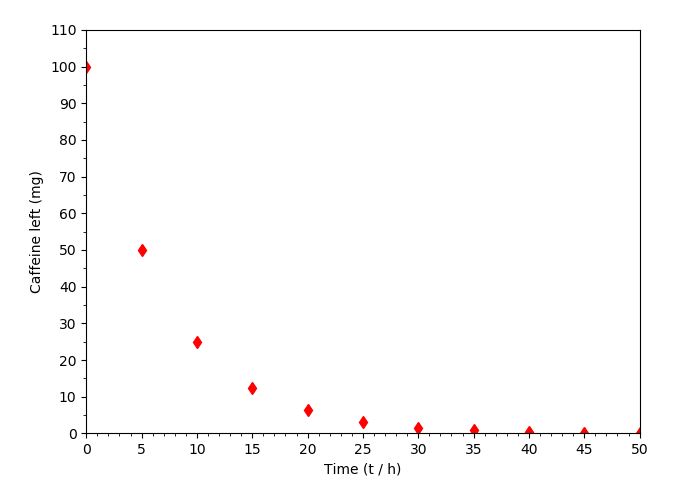
\includegraphics[scale=0.8]{table1.png}
                \end{center}

                But we'd like to draw a line of best fit on the graph, do do that we must use the points and data given to calculate. It's apparent that it's an exponential function due to its initial curve sloping down and getting closer and closer to zero. 

                \section{Determining a function}

                As discussed in the previous section, it seems like the data follows an exponential path, and since it's a downward sloping curve it's fair to assume that its exponent is negative.
                
                \noindent
                We can observe that the rate of decay is dependant on the amount of substance left. We can therefore assume that there's a proportionality between the initial amount of substance,$N_\Theta$, and the amount decayed, $N$. 

                \noindent 
                We can express this Mathematically as follows:
                
                        $$\frac{\delta N}{\delta t} = -\lambda N_\Theta $$

                Where $\frac{\delta N}{\delta t}$ is the change in the substance over a change in time, which is just another way of saying "How much decayed over X amount of time". This must be proportional to the initial amount of the substance, but for the proportionality to work out we need a \textit{proportionality constant}, which is this case is $\lambda$ (this is also known as the decay constant). 
                \noindent
                We know all the values except the decay constant, $\lambda$. This can be mathematically solved.


                \noindent
                By looking at our original equation we can see that it is possible to set it up as a \textit{differential equation} and integrate both sides, one integrating for $\delta N$ and one for $\delta t$
                        $$\frac{1}{N} \delta N_\Theta  = -\lambda \delta t$$

                        $$\int \frac{1}{N} \delta N_\Theta  = \int -\lambda \delta t$$
                        $$ ln(N) + c_1 = -\lambda t + c_2 $$
                        $$ ln(N)  = -\lambda t + c_3 $$
                \noindent
                We can the rearrange this to get $N$ as a function of $t$ by elevating the entire expression to the power of $e$:
                
                        $$ N(t) = e^{-\lambda t + c_3} $$

                Which can be re-written as:

                        $$ N(t) = e^{-\lambda t}e^{c_3} $$

                Since $c_3$ is an arbitrary constant, we can relabel the expression $e^{c_3}$ as a new constant called $c_4$, which gives us:

                        $$ N(t) = e^{-\lambda t}{c_4} $$

                At $t=0$ the compound has yet had a chance to decay, so we can also say that $N(0) = N_\Theta$, solving for $c_4$ then gives:
                
                        $$ N(0) = e^{-\lambda 0}{c_4} $$
                        $$ N(0) = 1 \times {c_4} $$
                        $$N(0) = N_\Theta = c_4$$

                We can then substitute that into ur function to get:   
                        $$ N(t) = N_\Theta e^{-\lambda t} $$

                %https://www.khanacademy.org/science/physics/quantum-physics/in-in-nuclei/v/exponential-decay-formula-proof-can-skip-involves-calculus

                This formula is often known as the "Exponential decay formula", which seems to fit our model knowledge caffeine well.

                \section{Our equation}
                As derived in the section above, our model for the decay of caffeine will follow the exponential decay formula.

                In our data, it is shown that the initial amount of caffeine is $100mg$ and that its half-life is $5 hours$. We can therefore sum up the values of our variables as follows,
                         $$N_\Theta = 100mg$$
                         $$N_1 = 50mg$$ 
                        $$t = 5 \times 60 = 300min$$
                        $$ \lambda = x$$
                        
               \noindent 
               and solve for $\lambda$. We re-arrange our function before we plug in the appropriate values:
                        $$ N(t) = N_\Theta e^{-\lambda t}$$
                        $$ ln(N) = ln(N_\Theta) -\lambda t $$
                        $$ \lambda = -\frac{ln(N)}{ln(N_\Theta)t}$$
                
                \noindent 
                Then substituting the appropriate values gives us:
                        $$\lambda = -\frac{ln(100)}{ln(50)\times 300} = -0.00392$$

                It is now possible to graph our model of the decay of caffeine.
                  
                \section{The Model}

                Here I'll make the best fit graph and determine when to drink coffee before bed etc

                        
                
                \pagebreak
                \section{Appendix}
                \inputminted{python}{decay.py} %yes

\end{document}

